\section{Curvature: coz being flat is boring!}
Let us start with the normal meaning of curvature. For a one dimensional curve, to actually see it is `curved', we need to visualise it in two dimension. Similarly, for two dimensional surface, to see its curvature, we need to embed it in three dimensional space. So, for an $n$ dimensional space, the curvature properties which require it to be embedded in a $n+1$ dimensions is called \textit{extrinsic curvature}.\\[0.3cm]
Now, imagine a 2D creature (someone from \textit{Flatland} perhaps) whose entirely life revolves in a 2D space, who doesn't have a taste for any other dimensions, how can that being say whether it is living in a flat space or curved space? One thing it can do is, it can just join three points with shortest distance lines and then measure the sum of the internal angles of the triangle. If they do not sum to $180^\circ$, then it is not a flatland. This is called \text{intrinsic curvature} property, since we are not leaving the space.
\subsection{Parallel Transport} 
\begin{figure}[H]
    \centering 
    \tikzset{every picture/.style={line width=0.75pt}} %set default line width to 0.75pt        

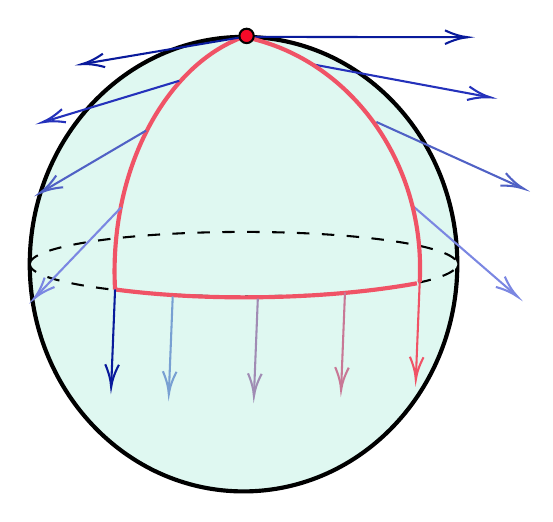
\begin{tikzpicture}[x=0.75pt,y=0.75pt,yscale=-1,xscale=1]
%uncomment if require: \path (0,300); %set diagram left start at 0, and has height of 300

% Define gradient colors
\definecolor{polecolor}{RGB}{9,26,155}
\definecolor{midcolor}{RGB}{80,97,197}
\definecolor{equatorcolor}{RGB}{240,83,102}

%Shape: Ellipse [id:dp46139127562543714] 
\draw  [fill={rgb, 255:red, 223; green, 248; blue, 241 }  ,fill opacity=1 ][line width=1.5]  (202,151.5) .. controls (202,91.02) and (248.11,42) .. (305,42) .. controls (361.89,42) and (408,91.02) .. (408,151.5) .. controls (408,211.98) and (361.89,261) .. (305,261) .. controls (248.11,261) and (202,211.98) .. (202,151.5) -- cycle ;
%Shape: Ellipse [id:dp931416204385338] 
\draw  [fill={rgb, 255:red, 223; green, 248; blue, 241 }  ,fill opacity=1 ][dash pattern={on 4.5pt off 4.5pt}] (202,151.5) .. controls (202,142.92) and (248.11,135.97) .. (305,135.97) .. controls (361.89,135.97) and (408,142.92) .. (408,151.5) .. controls (408,160.08) and (361.89,167.03) .. (305,167.03) .. controls (248.11,167.03) and (202,160.08) .. (202,151.5) -- cycle ;

%Straight Lines - Pole to equator (right side) - gradient from pole blue to equator red
\draw [color=polecolor ,draw opacity=1 ][fill={rgb, 255:red, 152; green, 241; blue, 241 }  ,fill opacity=1 ]   (305,42) -- (413,42.16) ;
\draw [shift={(413,42.17)}, rotate = 180.09] [color=polecolor ,draw opacity=1 ][line width=0.75]    (10.93,-3.29) .. controls (6.95,-1.4) and (3.31,-0.3) .. (0,0) .. controls (3.31,0.3) and (6.95,1.4) .. (10.93,3.29)   ;

\draw [color={rgb, 255:red, 36; green, 49; blue, 187 }  ,draw opacity=1 ][fill={rgb, 255:red, 152; green, 241; blue, 241 }  ,fill opacity=1 ]   (337,55) -- (422.03,70.8) ;
\draw [shift={(424,71.17)}, rotate = 190.53] [color={rgb, 255:red, 36; green, 49; blue, 187 }  ,draw opacity=1 ][line width=0.75]    (10.93,-3.29) .. controls (6.95,-1.4) and (3.31,-0.3) .. (0,0) .. controls (3.31,0.3) and (6.95,1.4) .. (10.93,3.29)   ;

\draw [color=midcolor  ,draw opacity=1 ][fill={rgb, 255:red, 152; green, 241; blue, 241 }  ,fill opacity=1 ]   (369,83) -- (438.18,114.34) ;
\draw [shift={(440,115.17)}, rotate = 204.37] [color=midcolor  ,draw opacity=1 ][line width=0.75]    (10.93,-3.29) .. controls (6.95,-1.4) and (3.31,-0.3) .. (0,0) .. controls (3.31,0.3) and (6.95,1.4) .. (10.93,3.29)   ;

\draw [color={rgb, 255:red, 123; green, 135; blue, 226 }  ,draw opacity=1 ][fill={rgb, 255:red, 152; green, 241; blue, 241 }  ,fill opacity=1 ]   (386,123) -- (435.49,165.86) ;
\draw [shift={(437,167.17)}, rotate = 220.89] [color={rgb, 255:red, 123; green, 135; blue, 226 }  ,draw opacity=1 ][line width=0.75]    (10.93,-3.29) .. controls (6.95,-1.4) and (3.31,-0.3) .. (0,0) .. controls (3.31,0.3) and (6.95,1.4) .. (10.93,3.29)   ;

%Shape: Arc [id:dp7516111540217032] 
\draw  [draw opacity=0][line width=1.5]  (305,42) .. controls (350.84,50.95) and (386.98,93.6) .. (389.87,146.73) .. controls (390.11,151.23) and (390.11,155.69) .. (389.88,160.08) -- (288.03,152.26) -- cycle ; \draw  [color=equatorcolor  ,draw opacity=1 ][line width=1.5]  (305,42) .. controls (350.84,50.95) and (386.98,93.6) .. (389.87,146.73) .. controls (390.11,151.23) and (390.11,155.69) .. (389.88,160.08) ;  
%Shape: Arc [id:dp5191253755043371] 
\draw  [draw opacity=0][line width=1.5]  (305,42) .. controls (271.82,54.02) and (245.85,95.51) .. (243.1,146.15) .. controls (242.77,152.1) and (242.78,157.97) .. (243.1,163.7) -- (321.69,150.42) -- cycle ; \draw  [color=equatorcolor  ,draw opacity=1 ][line width=1.5]  (305,42) .. controls (271.82,54.02) and (245.85,95.51) .. (243.1,146.15) .. controls (242.77,152.1) and (242.78,157.97) .. (243.1,163.7) ;  
%Shape: Arc [id:dp9510794372298369] 
\draw  [draw opacity=0][line width=1.5]  (388.53,160.73) .. controls (367.1,164.64) and (340.62,167.11) .. (311.93,167.45) .. controls (286.67,167.75) and (263.07,166.36) .. (243.1,163.7) -- (311.58,137.46) -- cycle ; \draw  [color=equatorcolor  ,draw opacity=1 ][line width=1.5]  (388.53,160.73) .. controls (367.1,164.64) and (340.62,167.11) .. (311.93,167.45) .. controls (286.67,167.75) and (263.07,166.36) .. (243.1,163.7) ;  

%Straight Lines - Equator to pole (downward) - gradient from equator red back to pole blue
\draw [color=equatorcolor ,draw opacity=1 ][fill={rgb, 255:red, 152; green, 241; blue, 241 }  ,fill opacity=1 ]   (389.88,160.08) -- (388.08,205.17) ;
\draw [shift={(388,207.17)}, rotate = 272.29] [color=equatorcolor ,draw opacity=1 ][line width=0.75]    (10.93,-3.29) .. controls (6.95,-1.4) and (3.31,-0.3) .. (0,0) .. controls (3.31,0.3) and (6.95,1.4) .. (10.93,3.29)   ;

\draw [color={rgb, 255:red, 200; green, 120; blue, 150 }  ,draw opacity=1 ][fill={rgb, 255:red, 152; green, 241; blue, 241 }  ,fill opacity=1 ]   (353.88,165.08) -- (352.08,210.17) ;
\draw [shift={(352,212.17)}, rotate = 272.29] [color={rgb, 255:red, 200; green, 120; blue, 150 }  ,draw opacity=1 ][line width=0.75]    (10.93,-3.29) .. controls (6.95,-1.4) and (3.31,-0.3) .. (0,0) .. controls (3.31,0.3) and (6.95,1.4) .. (10.93,3.29)   ;

\draw [color={rgb, 255:red, 160; green, 140; blue, 180 }  ,draw opacity=1 ][fill={rgb, 255:red, 152; green, 241; blue, 241 }  ,fill opacity=1 ]   (311.88,168.08) -- (310.08,213.17) ;
\draw [shift={(310,215.17)}, rotate = 272.29] [color={rgb, 255:red, 160; green, 140; blue, 180 }  ,draw opacity=1 ][line width=0.75]    (10.93,-3.29) .. controls (6.95,-1.4) and (3.31,-0.3) .. (0,0) .. controls (3.31,0.3) and (6.95,1.4) .. (10.93,3.29)   ;

\draw [color={rgb, 255:red, 120; green, 160; blue, 210 }  ,draw opacity=1 ][fill={rgb, 255:red, 152; green, 241; blue, 241 }  ,fill opacity=1 ]   (270.88,167.08) -- (269.08,212.17) ;
\draw [shift={(269,214.17)}, rotate = 272.29] [color={rgb, 255:red, 120; green, 160; blue, 210 }  ,draw opacity=1 ][line width=0.75]    (10.93,-3.29) .. controls (6.95,-1.4) and (3.31,-0.3) .. (0,0) .. controls (3.31,0.3) and (6.95,1.4) .. (10.93,3.29)   ;

\draw [color=polecolor ,draw opacity=1 ][fill={rgb, 255:red, 152; green, 241; blue, 241 }  ,fill opacity=1 ]   (243.1,163.7) -- (241.3,208.79) ;
\draw [shift={(241.22,210.79)}, rotate = 272.29] [color=polecolor ,draw opacity=1 ][line width=0.75]    (10.93,-3.29) .. controls (6.95,-1.4) and (3.31,-0.3) .. (0,0) .. controls (3.31,0.3) and (6.95,1.4) .. (10.93,3.29)   ;

%Straight Lines - Left side gradient (pole to equator, then back)
\draw [color={rgb, 255:red, 123; green, 135; blue, 226 }  ,draw opacity=1 ][fill={rgb, 255:red, 152; green, 241; blue, 241 }  ,fill opacity=1 ]   (246.04,124.16) -- (205.38,166.72) ;
\draw [shift={(204,168.17)}, rotate = 313.69] [color={rgb, 255:red, 123; green, 135; blue, 226 }  ,draw opacity=1 ][line width=0.75]    (10.93,-3.29) .. controls (6.95,-1.4) and (3.31,-0.3) .. (0,0) .. controls (3.31,0.3) and (6.95,1.4) .. (10.93,3.29)   ;

\draw [color=midcolor  ,draw opacity=1 ][fill={rgb, 255:red, 152; green, 241; blue, 241 }  ,fill opacity=1 ]   (258.04,87.16) -- (208.72,116.15) ;
\draw [shift={(207,117.17)}, rotate = 329.55] [color=midcolor  ,draw opacity=1 ][line width=0.75]    (10.93,-3.29) .. controls (6.95,-1.4) and (3.31,-0.3) .. (0,0) .. controls (3.31,0.3) and (6.95,1.4) .. (10.93,3.29)   ;

\draw [color={rgb, 255:red, 36; green, 49; blue, 187 }  ,draw opacity=1 ][fill={rgb, 255:red, 152; green, 241; blue, 241 }  ,fill opacity=1 ]   (274.04,63.16) -- (209.91,82.59) ;
\draw [shift={(208,83.17)}, rotate = 343.14] [color={rgb, 255:red, 36; green, 49; blue, 187 }  ,draw opacity=1 ][line width=0.75]    (10.93,-3.29) .. controls (6.95,-1.4) and (3.31,-0.3) .. (0,0) .. controls (3.31,0.3) and (6.95,1.4) .. (10.93,3.29)   ;

\draw [color=polecolor ,draw opacity=1 ][fill={rgb, 255:red, 152; green, 241; blue, 241 }  ,fill opacity=1 ]   (305,42) -- (228.97,54.83) ;
\draw [shift={(227,55.17)}, rotate = 350.42] [color=polecolor ,draw opacity=1 ][line width=0.75]    (10.93,-3.29) .. controls (6.95,-1.4) and (3.31,-0.3) .. (0,0) .. controls (3.31,0.3) and (6.95,1.4) .. (10.93,3.29)   ;

%Shape: Circle [id:dp08879929848455848] 
\draw  [color={rgb, 255:red, 0; green, 0; blue, 0 }  ,draw opacity=1 ][fill={rgb, 255:red, 245; green, 10; blue, 40 }  ,fill opacity=1 ] (303,41.53) .. controls (303,39.62) and (304.55,38.07) .. (306.47,38.07) .. controls (308.38,38.07) and (309.93,39.62) .. (309.93,41.53) .. controls (309.93,43.45) and (308.38,45) .. (306.47,45) .. controls (304.55,45) and (303,43.45) .. (303,41.53) -- cycle ;

\end{tikzpicture}

    \caption{Parallel Transport of a vector on a sphere (pardon the distorted diagram tho!). We can observe that a vector starting from a point on the sphere, after moving along the closed loop, does not remain the same vector. This is an important indication of curvature of space.}
\end{figure}
\subsection{Riemann Curvature Tensor}
